\begin{frame}{RIVET}
\begin{itemize}
\item<1-> Let's think about how this could go wrong and how we could fix it!
\item<2-> Suppose that, instead of data that look like this:
\begin{figure}
\begin{tikzpicture}[scale = 1.5]
    \draw plot[mark=*, mark size = 0.5, only marks] file {data/data3.txt};
\end{tikzpicture}
\end{figure} 
\end{itemize}
\end{frame}
%---------------------------------------------------------------
\begin{frame}{RIVET}
\begin{itemize}
\item Let's think about how this could go wrong and how we could fix it!
\item We had data that looked like this:
\begin{figure}
\begin{tikzpicture}[scale = 0.5]
    \draw plot[mark=*, mark size = 1.5, only marks] file {data/data7.txt};
\end{tikzpicture}
\end{figure} 
\end{itemize}
\end{frame}
%---------------------------------------------------------------
\begin{frame}{RIVET}
\begin{itemize}
\item<1-> This is a much more realistic example.
\item<2-> The blue points -- noise -- will make it hard to see the generator of $H_1$.
\begin{figure}
\begin{tikzpicture}[scale = 0.5]
    \draw plot[mark=*, mark size = 1.5, only marks] file {data/data7.txt};
    \draw[color = blue] plot[mark=*, mark size = 1.5, only marks] file {data/data7noise.txt};
\end{tikzpicture}
\end{figure} 
\end{itemize}
\end{frame}
%---------------------------------------------------------------
\begin{frame}{RIVET}
The first barcode includes the entire data set.  The second barcode eliminates the blue 'noise'.

\begin{figure}
\centering
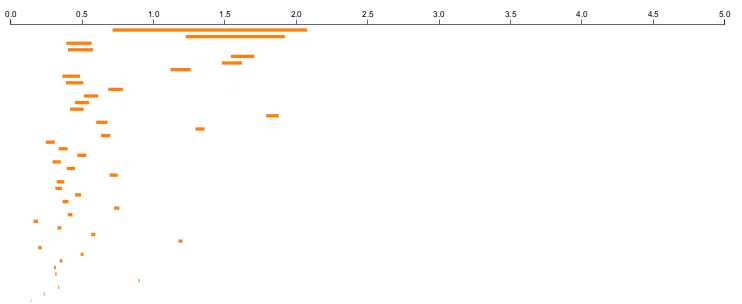
\includegraphics[scale=0.35]{images/data7.png}
\end{figure} 

\begin{figure}
\centering
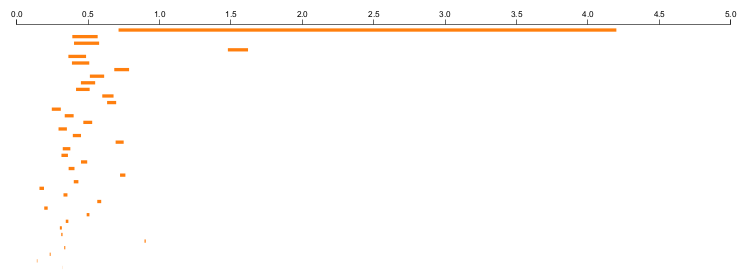
\includegraphics[scale=0.35]{images/data7nonoise.png}
\end{figure} 
\end{frame}
%---------------------------------------------------------------
\begin{frame}{RIVET}
\begin{itemize}
\item<1-> One way to deal with such situations: consider the density of the points.
\begin{figure}
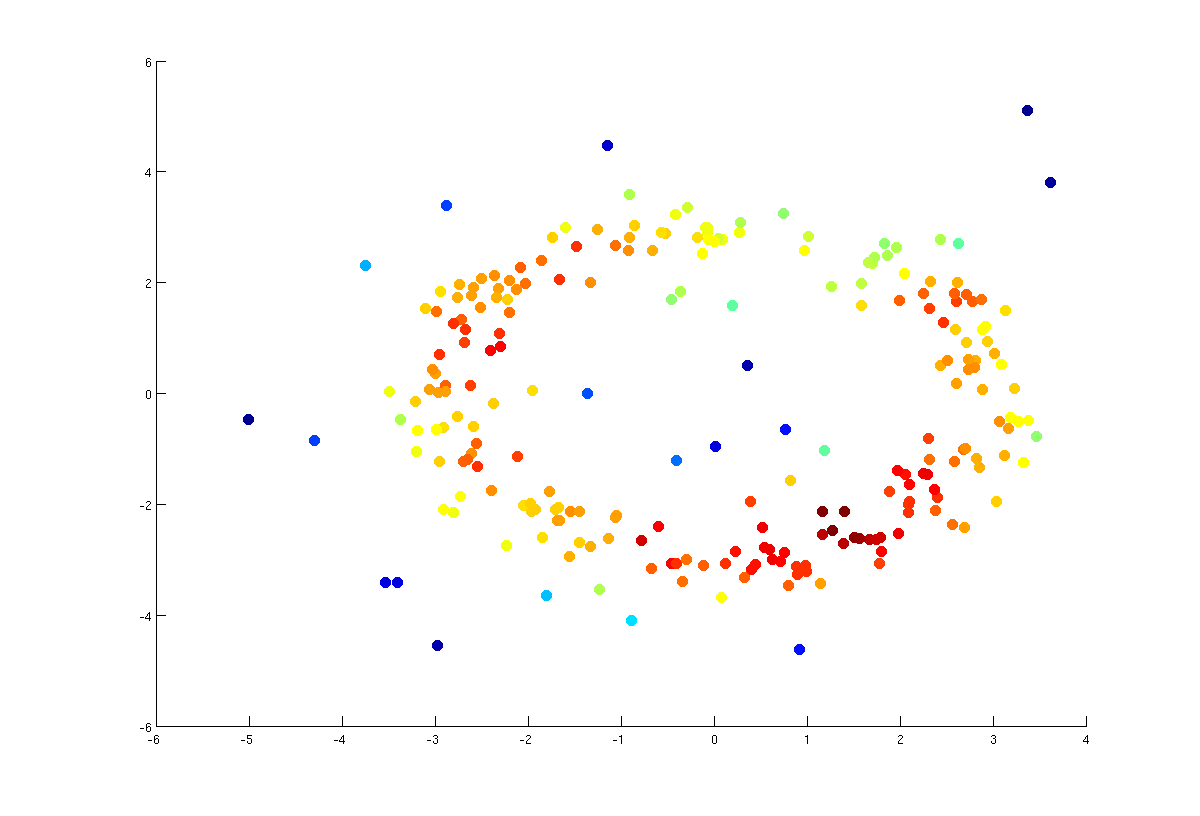
\includegraphics[scale=0.2]{images/data7density}
\caption{A density heat map of the data}
\end{figure} 
\item<2-> Letting the density threshold vary results in \textbf{multi-parameter persistence}!
\end{itemize}
\end{frame}
%---------------------------------------------------------------
\begin{frame}{RIVET}
\begin{itemize}
\item<1-> Michael Lesnick and Matthew Wright have written a program for visualizing multiparameter persistence.\cite{lesnick2015interactive}
\item<2-> Installation is not so simple -- let us go through it together!
\end{itemize}
\end{frame}